% Supporting Information for learned_sigma_profile.tex. Compiled with XeLaTeX, twice.
%
% SCOPE. This document holds the five items the article's "Supporting Information Available"
% section names, and nothing else. Each section below answers one of them, in that order.
% The rule for admission is that a section is either pointed to by the article or needed to
% reproduce a reported number; tools/check_si_contract.py enforces it.
%
% The Supporting Information of the previous submission (grounding_paradox_si.tex) belongs to
% a different argument and is left untouched.
\documentclass[journal=jcisd8,manuscript=suppinfo,layout=twocolumn]{achemso}
% =====================================================================
% SHARED PREAMBLE, \input by BOTH documents of this submission:
%   grounding_paradox.tex      the article                (manuscript=article)
%   grounding_paradox_si.tex   the Supporting Information (manuscript=suppinfo)
% Split out on 2026-08-02, when the Supporting Information became its own file at
% the request of all three referees and because ACS deposits it as a separate one.
% Everything here was the article's own preamble before the split and is unchanged
% apart from the xr-hyper line; the point of the file is that the two documents
% cannot drift apart -- a macro added for one is defined for both.
% What is NOT here, because it differs between the two: \documentclass (the
% manuscript type), the title/author/abstract block, \abbreviations, \keywords,
% \externaldocument (each document names the other), and the Supporting
% Information's S-numbering.
% =====================================================================
\SectionNumbersOn
\usepackage{amsmath,amssymb,amsthm}
\usepackage{array}
\usepackage{booktabs}
% Ragged-right paragraph column. Narrow justified p-columns in the claim and
% decomposition tables stretched a two-word line across the whole column; L{} sets the
% same text without the stretch, which is what let the column widths be rebalanced
% against actual content instead of against the worst justified line.
\newcolumntype{L}[1]{>{\raggedright\arraybackslash}p{#1}}
\usepackage{graphicx}
\usepackage{xcolor}
% ---------------------------------------------------------------------
% CROSS-DOCUMENT REFERENCES. The article and the Supporting Information are two
% separate documents, so neither LaTeX run can see the other's \label{}s. xr-hyper
% reads the other document's .aux and makes its labels resolve to the ordinary
% \ref, so not one of the 234 references that cross the boundary had to be rewritten
% as a hand-maintained plain-text pointer. The Supporting Information numbers itself
% S1, S2, ... (sections, tables, figures, equations, lemmas), so a resolved number
% says by itself which of the two documents it is in.
% xr-hyper, NOT xr: under hyperref \newlabel carries five arguments and plain xr
% reads the wrong one. It has to be loaded BEFORE hyperref, which is the only reason
% this line sits here and not beside \externaldocument.
% BUILD ORDER follows from it: the first pass of either document writes the .aux the
% other one reads, so from a clean directory it is xelatex on both, bibtex on both,
% then xelatex on both twice more. Building only one of the two from clean leaves
% its cross-document references as `??', and LaTeX reports that as a warning, not an
% error -- check the log for "There were undefined references", do not trust the
% exit status alone.
% ---------------------------------------------------------------------
\usepackage{xr-hyper}
% hidelinks: without it hyperref's default pdfborder={0 0 1} draws a rectangle around every
% cross-reference and citation. The boxes are invisible on screen in some viewers but print,
% and ACS production receives the PDF as-is.
\usepackage[hidelinks]{hyperref}

% ---------------------------------------------------------------------
% FLOAT PLACEMENT. In the two-column measure a deferred `table*'/`figure*' blocks every
% starred float after it, and stock LaTeX flushes that queue only at \clearpage -- which
% here is \end{document}. Left alone, every float from Table 2 onward printed after the
% bibliography, tens of pages from the text that cites it. dblfloatfix repairs the ordering
% and lets a double float reach the bottom of a column; the fractions below let a tall
% starred float be a top float instead of being sent to a float page. The starred floats that sit
% at that height limit additionally carry `p' in their own placement specifiers, so a float page is
% available to them and the queue never backs up; the note at each of them says so. Give a new tall
% `table*'/`figure*' the same `p'. Do NOT name those floats by number here: the numbering has moved
% twice as tables crossed between the two documents, and a stale number in this comment sends the
% next reader to the wrong float. Do NOT force the queue out with \afterpage{\clearpage} before Sec. 6.5
% or before the Discussion: in two-column mode that fires at a column boundary rather than a
% page boundary, so it ends the page with the right-hand column empty -- a blank half page
% before the Discussion -- and it buys no placement that `p' does not.
% Do not tighten these back without checking where the floats land.
% ---------------------------------------------------------------------
\usepackage{dblfloatfix}
\renewcommand{\topfraction}{0.92}
\renewcommand{\dbltopfraction}{0.92}
\renewcommand{\bottomfraction}{0.6}
\renewcommand{\textfraction}{0.06}
\renewcommand{\floatpagefraction}{0.6}
\renewcommand{\dblfloatpagefraction}{0.6}
\setcounter{topnumber}{3}
\setcounter{dbltopnumber}{3}
\setcounter{bottomnumber}{2}
\setcounter{totalnumber}{5}

\newtheorem{theorem}{Theorem}
\newtheorem{lemma}{Lemma}
\newtheorem{proposition}{Proposition}
\newtheorem{corollary}{Corollary}
\newtheorem{assumption}{Assumption}
\newtheorem{definition}{Definition}

% amsthm sets the optional argument of `proof' as a \trivlist label, i.e. one unbreakable
% \hbox. Four of the SI proof headers are longer than the two-column measure and ran into the
% neighbouring column. This redefinition is amsthm's own, with the head moved out of the label
% and into the paragraph so it wraps; \pushQED/\popQED and the spacing are unchanged.
\makeatletter
\renewenvironment{proof}[1][\proofname]{\par
  \pushQED{\qed}%
  \normalfont \topsep6\p@\@plus6\p@\relax
  \trivlist
  \item[]\hskip\labelsep{\itshape #1\@addpunct{.}}\enspace\ignorespaces
}{\popQED\endtrivlist\@endpefalse}
\makeatother

% ---------------------------------------------------------------------
% ACS-style lettered table footnotes. \tnk{a} sets the superscript key in the row or
% column head it qualifies; \tabnotes{...} sets the note block directly under the
% \bottomrule. THIS IS THE DESTINATION FOR CAPTION MATERIAL. A caption says what the
% table shows; anything that qualifies one row, one column or one cell is keyed to it
% here instead of being appended to the caption. Budget: <=40 words for a table
% caption, <=60 for a figure caption. Captions on this manuscript have been cut twice
% and grown back twice because each repair pass appended a sentence; if a finding
% needs an answer, put the answer in a note, in the body, or in the SI, and leave the
% caption alone.
% ---------------------------------------------------------------------
\newcommand{\tnk}[1]{\textsuperscript{\textit{#1}}}
\newcommand{\tabnotes}[1]{\par\vspace{2.5pt}\begingroup\footnotesize
  \setlength{\parindent}{0pt}\raggedright #1\par\endgroup}

% achemso sets the corresponding author's address with \url, which hyperref turns into a URI
% action with no scheme -- a viewer resolves "nikitapol@fbb.msu.ru" as a relative URL and the
% one external link in the PDF does not open a mail client. This is the class's own
% \acs@email@list@aux with \url replaced by an \href{mailto:...}; nothing else changes, and the
% printed form (\nolinkurl, in the class's \UrlFont) is identical.
\makeatletter
\newcommand*\acs@mailto[1]{\href{mailto:#1}{\nolinkurl{#1}}}
\renewcommand*\acs@email@list@aux{%
  \advance\@tempcnta\@ne\relax
  \ifnum\@tempcnta>\acs@author@cnt\relax\else
    \acs@ifundefined{@email@\@roman\@tempcnta}{}{%
      \advance\@tempcntb\@ne\relax
      \ifnum\@tempcntb>\@ne\relax
        ;
      \fi
      \expandafter\expandafter\expandafter\acs@mailto\expandafter
        \expandafter\expandafter{%
           \csname @email@\@roman\@tempcnta\endcsname
      }%
    }%
    \expandafter\acs@email@list@aux
  \fi
}
\makeatother

% ---------------------------------------------------------------------
% \pending marks a value that cannot be filled until submission. It used to set its argument in
% red bracketed monospace, which printed three conspicuous placeholders in a PDF otherwise ready to
% read. It now sets the argument as ordinary running text, so each sentence reads as a finished
% sentence and says in plain words when the value arrives; the MACRO ITSELF is the source marker,
% so `grep -n 'pending' paper/grounding_paradox.tex paper/sections/*.tex' still finds every one.
% STILL TO BE SUBSTITUTED BEFORE SUBMISSION (three call sites, all of them below):
%   1. grounding_paradox.tex, Data availability -- the git commit hash of the archived snapshot.
%      Minted last, when the snapshot is cut; replace \pending[hash to be supplied] with the hash.
%   2. grounding_paradox.tex, Data availability -- the Zenodo DOI. The deposit does not exist yet.
%   3. sections/SI.tex, compute ledger -- the same Zenodo DOI.
% The bold sentence in the Data availability statement, and limitation (x), both disclose that these
% are not yet real; do NOT delete either when the values are filled in -- rewrite them instead.
% ---------------------------------------------------------------------
% \pending prints in red so an unfilled field cannot be missed in a proof read. Three call sites:
%   Data availability -- the commit hash and the Zenodo DOI; App. I -- the same DOI.
% Both are minted at submission: the hash when the snapshot is cut, the DOI when the archive is
% published. Nothing else is outstanding; the repository itself is public.
\newcommand{\pending}[1][?]{{\color{red}\textbf{[#1]}}}
\newcommand{\lnx}{\ensuremath{\ln x_2}}
\newcommand{\Phicry}{\ensuremath{\Phi}}
\newcommand{\lng}{\ensuremath{\ln\gamma_2}}
\newcommand{\lngi}{\ensuremath{\ln\gamma_2^\infty}}
\newcommand{\Tm}{\ensuremath{T_m}}
\newcommand{\dHfus}{\ensuremath{\Delta H_{\mathrm{fus}}}}
\newcommand{\Rgas}{\ensuremath{R}}
\newcommand{\zstar}{\ensuremath{z^\star}}
\newcommand{\Bclos}{\ensuremath{B_{\mathrm{closure}}}}
\newcommand{\Binsuf}{\ensuremath{B_{\mathrm{insuff}}}}
\newcommand{\Ex}{\ensuremath{\mathbb{E}}}
\newcommand{\Var}{\ensuremath{\mathrm{Var}}}
% The grounding gap. Renamed from \Gamma (2026-07-27) so that it no longer collides with the
% COSMO-SAC segment activity coefficient \Gamma_S of Eq.~(4).
\newcommand{\Ggap}{\ensuremath{\mathcal{G}}}
% Hammett substituent constant, renamed from sigma so that it no longer collides with the
% charge-density profile sigma of the main text.
\newcommand{\hammett}{\ensuremath{\sigma_{\mathrm H}}}

% Line breaking. emergencystretch 2.5em with the default hyphenation penalties left 240 underfull
% boxes, 40 of them at badness 10000: loose lines that waste horizontal space. Allowing more
% hyphenation and less emergency stretch tightens them. Measured on the full document: 240 -> 202
% underfull, 0 overfull either way, and the main text loses a page (22 -> 21). Raising
% emergencystretch back to 2em restores the page; lowering hyphenpenalty below 50 starts to
% produce overfull boxes.
\setlength{\emergencystretch}{1.5em}
\tolerance=2000
\hyphenpenalty=50
\exhyphenpenalty=50
\doublehyphendemerits=2500

\externaldocument[][nocite]{learned_sigma_profile}

\title{Supporting Information: When a Learned $\sigma$-Profile Is Not One: Diagnosing the
Intermediate of a Physics-Embedded Solubility Model}

\author{N.~L. Polomoshnov}
\affiliation[MSU]{Faculty of Bioengineering and Bioinformatics, Lomonosov Moscow State
University, Moscow, Russia}
\alsoaffiliation[IBMC]{V.~N. Orekhovich Institute of Biomedical Chemistry, Moscow, Russia}
\email{nikitapol@fbb.msu.ru}
\author{A.~V. Rudik}
\affiliation[IBMC]{V.~N. Orekhovich Institute of Biomedical Chemistry, Moscow, Russia}

\begin{document}

\maketitle

\noindent This document supports the article in five parts, in the order its Supporting
Information section lists them: the architecture and the training schedule (\S\ref{si:arch}); the
data, the splits and the auxiliary supervision streams (\S\ref{si:data}); the reading rule declared
for each measurement before it was made, with its outcome (\S\ref{si:rules}); what the observations
leave undetermined, which is the premise the measurements rest on (\S\ref{si:unresolved}); and a
second system in which a linear free-energy relation stands in for the closure (\S\ref{si:second}).
Every number here is produced by a named script in the deposited repository from a named file in
it; the mapping is \texttt{MANIFEST.md} in that repository.

% Body of learned_sigma_profile_si.tex. Five sections, one per item of the article's
% "Supporting Information Available" list, in that order.

\section{Architecture and training}
\label{si:arch}

\begin{table*}[t]
\centering
{\footnotesize
\begin{tabular}{@{}llll@{}}
\toprule
quantity & value & quantity & value \\
\midrule
\multicolumn{2}{@{}l}{\itshape encoder} & \multicolumn{2}{l}{\itshape fixed points} \\
hidden width                    & $64$            & damping $\lambda$                      & $0.7$ \\
message-passing layers          & $3$             & segment activity, train / eval         & $16$ / $30$ \\
node / edge feature dimension   & $35$ / $8$      & phase equilibrium, train / eval        & $5$ / $20$ \\
set2set processing steps        & $3$             & \multicolumn{2}{l}{\itshape schedule} \\
cross-attention layers          & $3$             & epochs, phases $1$--$3$                & $30$ / $70$ / $10$ \\
pair representation dimension   & $512$           & learning rate, phase $1$               & $2.6\times10^{-4}$ \\
dropout                         & $0.012$         & learning rate, phase $2$               & $8.5\times10^{-5}$ \\
trainable parameters            & $5.40$\,M       & learning rate, phase $3$               & $8.5\times10^{-6}$ \\
\multicolumn{2}{@{}l}{\itshape closure} & optimiser                              & Adam \\
segment area $a_{\mathrm{eff}}$ & $7.5$           & weight decay                           & $5\times10^{-4}$ \\
misfit constant $\alpha'$       & $16466.72$      & gradient clipping                      & $2.0$ \\
bonding coefficient $c_{\mathrm{hb}}$ & $85580$   & batch size                             & $64$ \\
bonding cutoff $\sigma_{\mathrm{hb}}$ & $0.0084$  & \multicolumn{2}{l}{\itshape direct control} \\
coordination number $z$         & $10$            & dropout                                & $0.174$ \\
normalisers $r_0$ / $q_0$       & $66.69$ / $79.53$ & phase-$2$ learning rate              & $8.6\times10^{-4}$ \\
profile grid, bins              & $51$            & weight decay                           & $4.2\times10^{-5}$ \\
                                &                 & gradient clipping                      & $2.54$ \\
                                &                 & epochs                                 & $110$ \\
\bottomrule
\end{tabular}}
\caption{Architecture, closure constants and training hyperparameters of the five checkpoints of
record, and the four hyperparameters on which the direct control was tuned separately; values not
listed for the control are shared with the physics arm. Units: $a_{\mathrm{eff}}$ in \AA$^2$, the
misfit constant in kcal\,\AA$^4$\,mol$^{-1}$\,e$^{-2}$, the bonding cutoff in e\,\AA$^{-2}$, the
normalisers in \AA$^3$ and \AA$^2$; the profile grid spans $\pm0.025$\,e\,\AA$^{-2}$.}
\label{tab:si-hyper}
\end{table*}

\paragraph{The model.}
A shared message-passing encoder embeds the solute and the solvent graphs, with a two-layer
residual role-specific branch. A set2set readout pools each graph, the two pass through a
cross-attention block, and the pair representation
$[\,g_s,\,g_v,\,g_s\!\odot g_v,\,|g_s-g_v|\,]$ feeds both heads. Table~\ref{tab:si-hyper} gives the
widths, the depths, the closure constants and the training hyperparameters; it is the schedule the
five checkpoints of record were trained under.

The crystal head predicts $\Tm=100+600\,\mathrm{logistic}(\cdot)\in[100,700]$\,K and
$\dHfus=S_H\,\mathrm{softplus}(\cdot)$, giving the ideal term $\Phicry(T)$ of
equation~\eqref{eq:sle}; the group-contribution $\Tm$ prior is affine-calibrated on the training
split before entering the head. The $\sigma$-profile head is a feed-forward network on the same
pair representation, ending in a normalised non-negative vector of $51$ bins.

The repository carries two further encoder backbones, a graph transformer and a variant that splits
messages into dispersive, polar and hydrogen-bonding channels. Neither is used by any run reported
here, and no accuracy comparison between backbones is claimed.

\paragraph{The closure, and what it omits.}
The differentiable COSMO-SAC layer uses the standard VT-2005 / Lin--Sandler constants, with the
Staverman--Guggenheim normalisers and the profile grid as listed in Table~\ref{tab:si-hyper}.

The layer runs the residual, segment-activity part of COSMO-SAC alone. The
Staverman--Guggenheim combinatorial term, the contribution molecular size and shape make to the
activity coefficient, is omitted, because it is a function of cavity volume and area rather than of
the profile and so carries no information about the quantity under study. A substitution that
replaces the profile and leaves the combinatorial term in place would move both terms and the
attribution would not be clean.

Restoring the term would change some of the article's magnitudes and none of its signs. It vanishes
for a pair of a molecule with itself, so the reference-state violation of
Section~\ref{sec:refstate} is unaffected. It would change the magnitudes in
Sections~\ref{sec:cost} and~\ref{sec:attribution}, where the size of the effect is the result. It
needs molar volumes, which the source database carries but the extracted table used here does not,
and which the network could supply with a second scalar head beside the one that already predicts
cavity area; its omission is a choice made when the table was extracted rather than a constraint.

\paragraph{Two fixed points, and the iteration counts they are run at.}
The pipeline contains two nested fixed points, each with its own iteration count, and the counts
differ between training and evaluation.

The two counts and the damping are in Table~\ref{tab:si-hyper}. The phase-equilibrium fixed point
is the damped map
$x_2^{(k+1)}=\lambda\exp(-\Phicry(T)-\lng(x_2^{(k)},T))+(1-\lambda)x_2^{(k)}$, run at the same
$\lambda$ as the segment loop, which is one configuration field read by both.

A count is a free parameter between fitting and scoring, so a checkpoint scored at a count far from
the one it was fitted at is evaluated through an operator it was never fitted against. For the
checkpoints reported here the exposure is bounded directly. Table~\ref{tab:si-iter} sweeps the
segment count with weights and rows held fixed: converging the solver makes the learned arm
slightly \emph{worse}, over an interval $0.021$ wide, and moves the contrast between the two arms
by $-0.008$ between the evaluation count and the fixed point, $1.9\%$ of itself. That movement is
not a direction: three of five seeds carry its sign, the per-seed range $[-0.031,+0.002]$ spans
zero, and one seed carries almost all of it.

\begin{table}[t]
\centering
{\footnotesize
\begin{tabular}{@{}rrrr@{}}
\toprule
segment iterations & learned & substituted & contrast \\
\midrule
$8$   & $1.9155$ & $2.2300$ & $+0.3145$ \\
$16$  & $1.9195$ & $2.3061$ & $+0.3866$ \\
$30$  & $1.9275$ & $2.3356$ & $+0.4081$ \\
$100$ & $1.9362$ & $2.3370$ & $+0.4008$ \\
$300$ & $1.9364$ & $2.3368$ & $+0.4004$ \\
\bottomrule
\end{tabular}}
\caption{Seed-mean \lnx\ mean absolute error against the number of segment-activity iterations,
with weights and rows held fixed. The training count is $16$ and the evaluation count $30$; the
fixed point is reached by about $300$. Contrast is the substituted arm minus the learned one.}
\label{tab:si-iter}
\end{table}

The aggregate is insensitive because the per-row shifts cancel, not because they are small. At $30$
iterations the median row moves $5.9\times10^{-4}$ against the converged solve, its ninety-fifth
percentile $0.136$ and its worst row $2.03$ in \lnx. The two profiles also converge at different
rates, in the direction the asymmetry predicts: at $30$ iterations the segment residual is a median
$9.7\times10^{-4}$ with a ninety-fifth percentile of $0.038$ and a worst case of $0.073$ in \lngi\
on the tabulation, against $2.4\times10^{-3}$, $0.077$ and $0.162$ on the learned profile, so the
broader learned profile is about twice the slower wherever the residual is large. What the count
does reach is under-counting: at eight iterations the contrast reads $+0.31$, understating it by
$0.094$. The exposure is therefore a head scored \emph{below} the count it was fitted at, which is
not the configuration of any run reported here.

\paragraph{Optimisation and curriculum.}
Training is a fixed three-phase curriculum: $30$ epochs of auxiliary-property pretraining, $70$ of
full solid-liquid equilibrium training, and $10$ of low-rate stabilisation, at learning rates
$2.6\times10^{-4}$, $8.5\times10^{-5}$ and $8.5\times10^{-6}$. The optimiser is Adam with weight
decay $5\times10^{-4}$, gradient clipping at $2.0$ and batch size $64$.

The direct control shares the encoder, interaction and readout verbatim and emits \lnx\ directly,
with a thermometer encoding of temperature in place of the dependence the physics arm receives
through $\Phicry(T)$ and the closure. It was tuned separately: dropout $0.174$ against $0.012$,
second-phase learning rate $8.6\times10^{-4}$ against $8.5\times10^{-5}$, weight decay
$4.2\times10^{-5}$ against $5\times10^{-4}$, gradient clipping $2.54$ against $2.0$, over $110$
epochs equal to the physics arm's total budget at the same width and depth. Width, depth, batch
size and epoch budget are matched and the optimisation is not, so any difference between the two
arms is a difference between two separately tuned pipelines and is not attributable to the
thermodynamic bottleneck alone. A hyperparameter-matched control was not run.

\paragraph{Objective.}
The objective is a weighted sum. Its registry holds $32$ terms, of which $17$ are hard-wired to
zero and two more default to zero through the configuration: disabled experimental scaffolding,
released with the code so that a reader of the configuration can see what is off.
Table~\ref{tab:si-loss} lists the terms carrying a non-zero default weight, together with the
$\sigma$-profile earth-mover term, which is applied outside the registry when the grounding stream
is on. Per-phase weight overrides are pinned in each run's resolved configuration, which is
deposited with the checkpoint.

One entry in that table is a diagnostic rather than a penalty. The monotonicity term
differentiates \lnx\ with respect to temperature without retaining a graph, so it enters
the reported objective and no gradient: varying only its weight moves the reported total
and leaves every parameter gradient unchanged. Its logged value was $0$ at every
evaluation, and a randomly initialised model scores $0$ as well, so that zero records the
construction and not the training --- $\lnx = -\Phicry(T) - \lng$ is non-decreasing in $T$
along the solver path wherever $\Phicry$ falls with $T$. Monotonicity in $T$ is carried
instead by the same-pair temperature-ranking and local van't Hoff terms, which are zero by
registry default and enabled only by the per-phase overrides, so they do not appear among
the defaults above.

\begin{table*}[t]
\centering
{\footnotesize
\begin{tabular}{@{}llr@{}}
\toprule
role & term & default wt. \\
\midrule
task                  & solubility (bin-weighted Huber on \lnx)   & $1.0$ \\
crystal grounding     & melting point $\Tm$                       & $0.3$ \\
                      & fusion enthalpy $\dHfus$                  & $0.3$ \\
activity grounding    & infinite-dilution \lngi                   & $0.5$ \\
                      & finite-composition \lng                   & $0.5$ \\
                      & Hansen parameters                         & $0.2$ \\
                      & $\sigma$-profile earth-mover              & stream \\
regulariser           & physics preference                        & $0.1$ \\
                      & adaptive-correction residual              & $0.01$ \\
                      & NRTL $\tau$                               & $0.01$ \\
control coupling      & direct-arm negative log-likelihood        & $0.2$ \\
                      & direct-arm regulariser                    & $0.05$ \\
architecture          & mixture-of-experts balance                & $0.02$ \\
diagnostic            & solubility monotonicity in $T$            & $0.1$ \\
\bottomrule
\end{tabular}}
\caption{Loss terms with a non-zero default weight. The $\sigma$-profile earth-mover term is not a
registry entry and is active only while the grounding stream is on. A further $17$ registered terms
are hard-wired to zero. The monotonicity entry carries a weight but no gradient, and is listed as a
diagnostic for that reason.}
\label{tab:si-loss}
\end{table*}

\paragraph{The activity-model variants that are not reported.}
The code implements two further activity models as controls: a fitted NRTL excess-Gibbs-energy
model, and its symmetric one-parameter collapse in which the two interaction parameters are tied to
a single predicted $\lngi$. Neither is used by any measurement in the article, which concerns the
$\sigma$-profile and therefore requires the profile-based closure. Their weights were not retained,
and no comparison between them and the COSMO-SAC arms is made here: the arms were separately tuned,
and a difference between separately tuned pipelines is not a property of the activity model.


\section{Data, splits and the auxiliary supervision streams}
\label{si:data}

\paragraph{Sources.}
Solubility is BigSolDB~2.0 \cite{krasnov2025bigsoldb}. Crystal $\Tm$ and $\dHfus$ come from an open
melting-point pool together with a group-contribution prior; melting-point tables are auto-detected
as degrees Celsius or kelvin, because a double conversion of an already-absolute table shifts every
$\Tm$ by $+273$\,K and $\Tm$ enters the ideal term directly. Reference $\sigma$-profiles are the
VT-2005 compilation \cite{mullins2006} as redistributed with Ref.~\cite{bell2020cosmosac}, ingested
to $1432$ compounds together with the COSMO cavity volume. Infinite-dilution activity coefficients
are from ThermoML \cite{frenkel2011thermoml}. The acid-dissociation data of \S\ref{si:second} are
the OPERA compilation \cite{mansouri2019opera}, $7904$ records, from which a uniform
net-formal-charge filter leaves $1004$ rows amenable to a Hammett treatment, $158$ meta or para and
$846$ ortho or heteroaromatic.

The reference profiles are computed for a single conformer and protonation state. Mismatch between
that state and the one a measurement was made in is error in the reference, and it is not signed:
it displaces the quantity every departure in the article is measured against. The article therefore
compares the learned profile with one tabulation throughout and makes no claim about the tabulation
itself.

\paragraph{Coverage, and why the matched set is small.}
The set on which a learned profile and a reference profile can both be scored against a measured
activity coefficient is limited by the intersection of the two, not by either alone. At $298$\,K it
holds $85$ pairs over $46$ solutes and $19$ solvents, and matching on RDKit canonical SMILES and on
InChIKey return the same set. They did not always. A standard InChI whose mobile-hydrogen layer
leaves the tautomer open was being resolved to a minor form, so formamide entered as the imidic
acid, N-methylformamide likewise and caprolactam as the lactim, and $27$ records then failed to
match a profile that was present under the amide form. That is not a tautomer crossed in the
matching but one introduced in our own conversion, since the records' InChI identifies the amide;
the conversion is corrected, the two rules agree, and this work therefore reports no trade-off
between them. The article uses the canonical-SMILES rule because it is the rule the deployed
$\sigma$-oracle uses.

Whether a larger database would enlarge that set is measured here rather than inferred from the
solute margin alone. Against PubChemQC COSMO, the largest open $\sigma$-profile database at
$334714$ distinct molecules, which is $148$ times the deposited compound list, joint coverage of
the $5608$ labelled test rows grows from $437$ rows over $11$ of the $147$ test solutes to $941$
rows over $23$. A pool $148$ times larger buys a matched set $2.2$ times larger, and the limit is
structural rather than accidental: that database stops below $250$\,Da and $19$ heavy atoms, while
the $124$ test solutes it does not hold carry a median of $25$ heavy atoms against $14$ for the
$23$ it does. The binding side is the solute. Of the labelled rows $4496$ fail on the solute alone
while $60$ of the $70$ test solvents are covered, so a database of this kind supplies the solvent
channel and leaves the drug-like solutes to be computed.

\paragraph{The split.}
The split is by Bemis--Murcko scaffold \cite{bemis1996}: molecules are grouped by ring system plus
linker with side chains stripped, and no scaffold appears in more than one partition. Every test
metric in the article is computed on the $5608$ labelled test rows, which span $147$ solutes.

The seeded split is not stable across versions of the data-preparation code. Regenerating it
reshuffles which scaffolds land in the test partition, which orphans every checkpoint and every
number measured on the previous split. All numbers in this work are therefore computed on a single
pinned split, whose per-file SHA-256 each run manifest records and whose files are deposited with
the checkpoints rather than regenerated.

\paragraph{The auxiliary supervision streams.}
An auxiliary stream is a sidecar table in the processed-dataset format whose rows are
self-solvent, carry no solubility label, and switch on the mask of one target only. Two streams
feed the runs reported here: a crystal stream carrying melting points, and a $\sigma$-profile
stream carrying reference profiles. A stream builder applies two guards and reports both in its
build summary. The first excludes any pool molecule whose Bemis--Murcko scaffold appears in the
validation or test partition, and aborts rather than proceed if a split file is missing. The second
reports how many pool molecules are not already labelled for that target in the training partition,
by canonical SMILES, because a stream that is mostly duplicates tests nothing and the null it
produces would be read as evidence that grounding does not help.

\paragraph{One build violated the first guard, and the exposure it leaves.}
A correct build of the $\sigma$-stream retains $1319$ of the $1427$ VT-2005 molecules that parse
into the pool; the stream file was at one point rebuilt with the exclusion pointed at the splits of
a small debug dataset, and that build carries $106$ rows whose scaffold is in the real test and
validation union, $91$ of them held-out solutes by canonical SMILES. What a leak can act on is the
labelled test set, and there the exposure is smaller: of the $147$ labelled test solutes, $7$ have
their own reference profile in the defective stream and $8$ have a scaffold relative in it ($297$
and $351$ of the $5608$ rows, $5.3\%$ and $6.3\%$), and for a scaffold split that solute coverage
rather than the row fraction is the load-bearing statistic. The correctly guarded build leaves none of either, and the crystal
stream's build on disk records the correct exclusion, so among the streams feeding these runs the
defect is confined to the $\sigma$ one. Per-run stream provenance was not logged, so the deposited
artifacts cannot certify which build fed which arm and the above is a bound rather than an
attribution; the runner now records the stream hash alongside the split hash.

\paragraph{Compute and determinism.}
The five checkpoints of record were trained on one machine from one commit, at seeds $42$ to $46$;
each manifest records the commit, the configuration, the seed and the environment. Retraining the
same arm on a different GPU architecture does not reproduce a checkpoint to within seed spread, so
a comparison of two checkpoints should be read against the hardware each was trained on. Analysis
is deterministic given a checkpoint and a seed, and every quantity reported in the article is a
median or a range over the five seeds.



\section{The control for each measurement}
\label{si:rules}

A contrast of this kind is interpretable only against something that would have come out
differently had the instrument been responding to something else. This section states, for each
row of Table~\ref{tab:battery}, what that control is and what outcome from it would have refuted
the reading. Each control is part of the measurement: the script that produces a deposit computes
its control in the same pass, over the same rows and the same weights, so the two cannot drift
apart. None of these is a pre-registration, with the one exception named at the end.

\paragraph{Does the observable determine the $\sigma$-profile?}
Control: the same Jacobian spectrum computed on random profiles carrying the same total area. The
reading is that the deficiency belongs to the closure as a map rather than to the trained head, so
it is the control's \emph{agreement} that supports it. A control resolving materially more
directions than the learned profile would refute it, because the restriction would then be
something the head does. The learned profiles give a median of two directions of fifty for $99\%$
of the information, range one to five; the random profiles give two.

\paragraph{Does the observable determine the crystal term?}
Control: the same Cram\'er--Rao bound recomputed with the melting temperature and the enthalpy of
fusion supplied as independent labels. A bound already tight without them would refute the reading.
It is $\pm20$\,kJ\,mol$^{-1}$ without and $\pm1.7$ with.

\paragraph{Does the head use the freedom?}
Control: the share of the molecule's cavity surface each charge-density window holds. A residual
distributed in proportion to area, that is an enrichment near one in every window, would refute the
reading that the departure is directed. Over the $71$ molecules of the clean pool the enrichment is
$3.97$ in the donor window, $2.03$ in the acceptor window and $0.88$ in the nonpolar core as
solute, and $3.78$, $1.96$ and $0.89$ as solvent.

\paragraph{Is the output layer responsible?}
Two controls, because the claim is negative and a negative needs both. The first is the smallest
bin mass the same head reaches anywhere, which bounds what the normalisation makes impossible; the
second is an untrained head of the same architecture, which gives the pedestal the parameterisation
produces before any data. A head unable to go far below its pedestal, or an untrained head whose
pedestal matched the trained one, would refute the reading. The head reaches $10^{-11}$, and the
untrained pedestal is a median $0.571$ against $0.02$ to $0.03$ trained.

\paragraph{Is the reference state preserved?}
Control: the same calculation with one profile supplied on both sides, which returns zero
identically. A control returning anything other than zero would place the deviation in the closure
rather than in the model, and would refute the reading. It returns zero exactly; the model's own
two role profiles give a median $|\lng|$ between $0.012$ and $0.044$ across seeds, largest $0.80$.

\paragraph{What does misplaced mass cost, and where?}
Control: the same per-bin sweep on random profiles of the same total area, which gives the
edge-to-core ratio a smooth object produces with no chemistry in it. A real-profile ratio inside
the random profiles' would refute the reading that the cost map is a property of the closure's
chemistry. The real ratios are $21\times$ and $15\times$ on the two row sets against $1.6\times$
random.

\paragraph{Does the intermediate decompose?}
Control: a randomly chosen part of the grid of the same size as the part being substituted, twenty
draws per seed. If substituting a random part were never worse than substituting none, the parts
would add and a per-bin attribution would be defined. A random third is worse than the fully
learned profile in $20\%$ of the $20\times5$ draws.

\paragraph{Where does the error that reaches the closure live?}
Controls: exact zeros written into the bins where the reference is zero, and a random third of the
grid, twenty draws per seed. A zero-bin repair recovering a share comparable to the nonzero-bin
repair would refute the reading that the consequential error is in the occupied bins. The nonzero
repair recovers $+89\%$ of the gap and the zero repair $-9\%$.

\paragraph{What does supplying the reference profile do?}
Control: the rows in which no profile is replaced because neither component is tabulated, which
must not move. Movement there would mean the substitution was reaching rows it does not touch and
would refute every number read from this contrast. Those rows move by less than
$4\times10^{-6}$. The activity coefficients improve from $1.75\pm0.06$ to $0.76$ and the solubility
worsens by $0.43\pm0.04$ over $5274$ rows.

\paragraph{The one measurement with a rule written beforehand.}
The reference-state test was prompted by a reviewer's observation that a role-dependent profile
would break $\gamma(i\ \mathrm{in}\ i)=1$. A rule was committed before the quantity was computed,
six minutes before the result in the repository history, and it reads as follows. The existing
closure validation cannot see the effect, because it supplies one tabulated profile to both sides
and so tests the closure rather than the model; under equal profiles $\gamma=1$ holds by
construction. The model is built with a role-specific branch, so one molecule receives different
profiles in the two slots, and the quantity to compute is therefore $\lngi$ with the solute-role
profile in one argument and the solvent-role profile in the other, at $298.15$\,K, with the layer's
default configuration. The declared control was the one-profile calculation, which must return zero
exactly; the declared refutation was that control returning anything else, in which case the
deviation would be the closure's. Both parts were then computed, and both came out as declared.

\section{What the observations leave undetermined}
\label{si:unresolved}

Section~\ref{sec:determined} of the article states the result: two of the fifty directions in which
a $\sigma$-profile can move carry $99\%$ of the information a solubility observation supplies, and
random profiles of equal area give the same count. This section gives what the article does not:
the protocol, the chemical locus of the directions that are resolved, an independent measurement at
infinite dilution, and the limits that travel with it.

\paragraph{Protocol, and why the control agreeing is the result.}
Fix the weights and the rows and perturb the $\sigma$-profile along each of the $51$ grid
coordinates in turn, recording the response of $\lng$; the information matrix is the Gram matrix of
the resulting Jacobian, and the reported count is the number of eigenvalues needed to carry $99\%$
of its trace. The control is the same construction on random profiles of equal total area. Its
agreement is the finding rather than a failure of the test: the deficiency belongs to the closure
as a map from a $51$-bin histogram to one number, so an observation of $\lng$ constrains a
two-dimensional shadow of the profile whatever profile is supplied, and what the head places in the
remaining coordinates is not decided by fitting.

\paragraph{Which directions are resolved.}
The resolved direction has a chemical locus as well as a rank. The dominant eigenvector
concentrates on the extreme-$|\sigma|$ bins on which the closure's hydrogen-bonding term acts, so
the coordinates the observation leaves free are the nonpolar and weakly polar interior of the
profile. The two measurements in the article meet here: the free coordinates are also the ones in
which misplaced mass is cheapest (Section~\ref{sec:cost}), so the network is least constrained
exactly where departures matter least, and the departure that does reach the thermodynamics is a
departure in magnitude rather than in location (Section~\ref{sec:attribution}).

\paragraph{The same picture at infinite dilution.}
A complementary measurement reaches it by another route. The aggregate activity Fisher matrix
$J^{\top}J$ with $J=\partial\lngi/\partial\sigma$ is rank one, and the per-molecule Fisher that
governs an individual profile has participation ratio about $1.4$ of $51$ even at full solvent
coverage.

Three limits travel with these numbers. The participation ratio is a concentration statistic and
not an exact count of resolved directions. It must be read against a permuted control rather than
absolutely, because finite differences decorrelate the redundant flat-profile coordinates and
inflate it. And it is measured at infinite dilution, so its transfer to the finite-composition
regime is not established here. None of this says that recovering the tabulated profile is
impossible in principle; it says the solubility observations do not require it.

\paragraph{Why the crystal term is treated differently.}
The article reports the condition number of the four-parameter fit and the Cram\'er--Rao bound it
implies. What follows for the design is the asymmetry between the two heads: the crystal term is
indeterminate from solubility alone but has an external label that closes the indeterminacy, which
is why it is supervised externally, whereas the profile coordinates the closure cannot see have no
such label. That asymmetry is the reason the article's question is about the profile rather than
the crystal term.


\section{A second system: a linear free-energy relation}
\label{si:second}

The article's measurements are made on one pipeline with one closure, so they cannot say whether
the behaviour depends on the closure's adequacy. This section reports a second system built so
that adequacy varies by chemical stratum and is known from structure alone.

\paragraph{Construction.}
The closure is a fixed Hammett linear free-energy relation,
$g=\mathrm{p}K_{a,0}-\rho\,\hammett^{\star}$, over a reaction series $s$, which fixes the
per-scaffold Hansch--Leo--Taft constants $(\mathrm{p}K_{a,0},\rho)$, and a substituent constant
$\hammett^{\star}$. A network predicts $\hammett^{\star}$ from structure and the prediction is
pushed through the fixed relation, which is the same arrangement as a $\sigma$-profile pushed
through COSMO-SAC. The tabulated Hansch--Leo values are the external reference for the predicted
coordinate, exactly as the VT-2005 table is for the profile. The constant carries its subscript
throughout so that it is not confused with the screening-charge density of the article.

Assignment is mechanical and reads structure only. Four reaction series are tried in the fixed
order benzoic acid, phenol, anilinium, pyridinium, and a record enters under the first whose
ionizing group matches exactly once, at a ring atom lying in exactly one six-membered aromatic
ring. Ring positions are typed by shortest ring-bond distance from that atom: one bond ortho, two
meta, three para. The constant $\hammett^{\star}$ is the sum over substituted positions of the
tabulated Hansch--Leo value for that substituent at that position, from a fixed list of nineteen;
an unsubstituted parent has $\hammett^{\star}=0$.

\paragraph{Why adequacy varies, and how the strata are defined.}
The two classical failure modes of a Hammett relation fall on either side of the distinction the
article draws. Resonance saturation is a curvature in the substituent constant that a linear
relation structurally cannot represent: a defect of the map. Ortho and steric field effects are
absent from the tabulated constants altogether: information the intermediate does not carry.

The strata follow from that. A record whose every substituted position is meta or para with a
tabulated substituent lies where the relation is close to exact. A record carrying an ortho
substituent, or one outside the tabulated list, lies where it is not; both enter $\hammett^{\star}$
as zero. The rule is a function of structure and never reads a residual, so the strata cannot be
chosen by outcome.


\paragraph{The same distinction, dialled continuously.}
Before the comparison on measured data, the two failure modes can be separated by construction.
Figure~\ref{fig:si-pka} dials each of them on a semi-synthetic Hammett series whose true values are
known in closed form, so that the cost of supplying the reference can be read against a quantity
that is not estimated. Degrading the relation while the constant stays sufficient makes the cost
follow the relation's own error, from $-0.03$ where the relation is exact to $+0.69$ where it is
not, against the relation's own $0.81$. Keeping the relation exact and starving the constant
instead leaves the relation's own error at zero throughout, and the cost still rises, from $-0.03$
to $+0.34$, crossing zero between fractions of $0.15$ and $0.30$. Supplying the reference is therefore costly
for two separable reasons, and only one of them is a defect of the map.

\begin{figure*}[t]
\centering
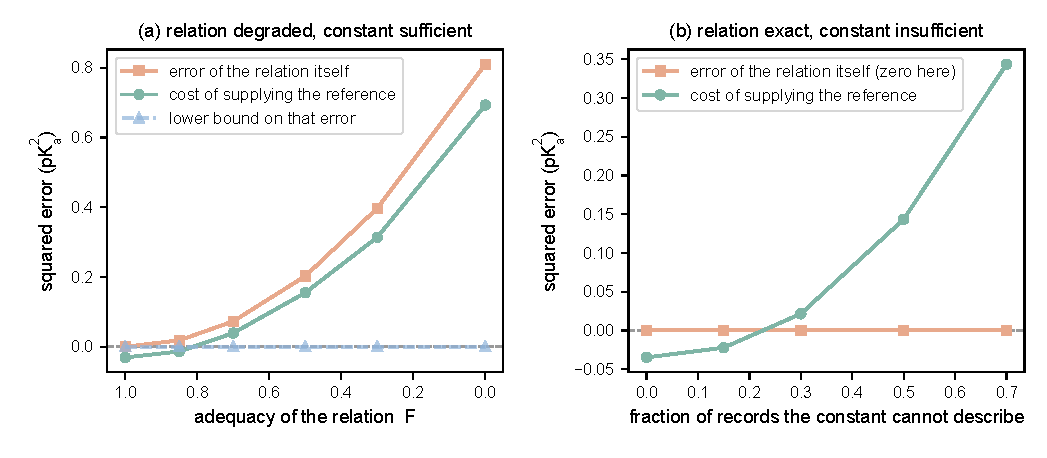
\includegraphics[width=\linewidth]{figs/fig_pka_hammett.pdf}
\caption{The two failure modes dialled directly, on a semi-synthetic Hammett series whose true
values are known in closed form. The cost of supplying the reference is the squared error obtained
with the tabulated constant minus that of the best free fit, so a positive value means supplying
the reference makes the prediction worse. (a) The relation is degraded while the constant stays
sufficient; adequacy $F$ falls from left to right. The cost tracks the relation's own error and
changes sign where the relation becomes adequate. (b) The relation is kept exact while a growing
fraction of records carries an effect the tabulated constant cannot describe. The relation's own
error is zero throughout and the cost still rises, so a cost of supplying the reference is not by
itself evidence that the relation is wrong.}
\label{fig:si-pka}
\end{figure*}

\paragraph{Data and one uniform filter.}
The source is the OPERA compilation \cite{mansouri2019opera}, $7904$ records. A small number are
supplied as pre-ionized microstates, inconsistent with a neutral-scaffold Hammett assignment, and
they degrade the well-specified stratum severely. They are removed by one rule applied uniformly to
both strata, net formal charge different from zero, which never references a residual and so cannot
be circular, and which keeps net-neutral substituents such as nitro. The filter removes $5$ of
$163$ rows in the well-specified stratum and $352$ of $1198$ in the other, leaving $1004$
Hammett-amenable rows, $158$ and $846$.

\paragraph{The comparison, and the result.}
The physics arm, encoder to $\hat{\hammett}$ to the fixed relation, is trained on $K=20$ stratified
within-scaffold splits, and the per-molecule error is paired against the deterministic reference
arm, stratum by stratum. Where the relation is well specified the reference wins: learned MAE
$0.48\pm0.09$ against $0.315\pm0.07$, a gap of $-0.165$, the reference better in $19$ of $20$
splits. Where it is not, the reference loses: learned $0.83\pm0.07$ against $1.62\pm0.08$, a gap of
$+0.79$, the reference worse in $20$ of $20$ splits.

The sign of the effect of supplying the true intermediate therefore follows the adequacy of the
relation it is supplied to, within one system, under one protocol, with the strata fixed by
structure.

\paragraph{Three limits.}
The comparison is within distribution. The companion run on a Bemis--Murcko scaffold split is
deposited beside it, and there nothing flips: both arms degrade and the learned arm degrades
further, so the reference helps on both strata. The reason the main comparison is not run on a
scaffold split is that such a split collapses the well-specified stratum to two ring systems. Every
solubility result in the article is measured on a scaffold split, so this is the one place the
protocol differs.

The resampling unit is the reaction series and only four exist, so the cluster bootstrap has $35$
distinct outcomes and a finest atom of about $0.004$. The interval endpoints quoted above are
percentiles of that law and are no finer; read as a sign test on four units the two statements are
$p=1/16$ and $p\approx0.31$. What the result rests on is the consistency of the sign across splits
and series and the size of the gap in the misspecified stratum, $+0.79$ against a reference error
of $1.62$, and not on a $P$ value. The refit that would settle the series-level question at four
units was not run.

Finally, a competence sweep over training fractions $1.0$, $0.5$, $0.25$ and $0.12$, six seeds
each, shows that the reference side of the comparison is fixed by the stratum and not by the data
budget: its error is the same at every budget while the learned side moves. In the well-specified
stratum the learned arm rises from $0.46$ to $0.98$ and never reaches the reference's $0.31$, so
the reference helps throughout. In the other it stays below the reference's $1.62$ across the whole
range, $0.85$ at full data and $1.31$ at $12\%$, so the reference hurts throughout. Only scaffold
extrapolation, where the predicted constant breaks down to $2.6\pm2.0$, pushes it back above and
reverts the sign, and that reversion is a property of the mean over six splits rather than of each:
three of the six still have the reference hurting, and the negative mean is carried by two splits.


\bibliography{references_verified}

\end{document}
